\chapter{Giới thiệu}
\label{Chapter1}

\section{Thông tin nhóm}

\begin{itemize}
    \item 22110215 - Phạm Thị Anh Thư
    \item 22110177 - Phạm Đăng Quang
    \item 22110204 - Nguyễn Thiện Thanh
    \item 22110210 - Võ Xuân Thiện
    \item 22110208 - Nguyễn Ngọc Thiện
\end{itemize}

\section{Mô hình ngôn ngữ lớn}
Ngày 30 tháng 11 năm 2022 đánh dấu một chương quan trọng trong lịch sử của học máy. Đó là ngày OpenAI phát hành ChatGPT, thiết lập một tiêu chuẩn mới cho chatbot được hỗ trợ bởi các Mô hình Ngôn ngữ Lớn và mang đến cho công chúng một trải nghiệm trò chuyện chưa từng có.

Kể từ đó, các mô hình ngôn ngữ lớn - còn được gọi là LLM - đã được công chúng chú ý do số lượng lớn các tác vụ mà chúng có thể thực hiện. Ví dụ bao gồm:
\begin{itemize}

    \item Tóm tắt văn bản: Các mô hình này có thể thực hiện việc tóm tắt các văn bản lớn, bao gồm văn bản pháp lý, đánh giá, hội thoại và nhiều văn bản khác.

    \item Phân tích cảm xúc: Chúng có thể đọc qua các đánh giá về sản phẩm và dịch vụ và phân loại chúng là tích cực, tiêu cực hoặc trung lập. Chúng cũng có thể được sử dụng trong Tài chính để xem liệu công chúng nói chung cảm thấy lạc quan hay bi quan về một số chứng khoán nhất định.

    \item Dịch ngôn ngữ: Chúng có thể cung cấp bản dịch theo thời gian thực từ ngôn ngữ này sang ngôn ngữ khác.

    \item Hệ thống đề xuất dựa trên văn bản: Chúng cũng có thể đề xuất các sản phẩm mới cho khách hàng dựa trên đánh giá của họ về các sản phẩm đã mua trước đó.
\end{itemize}

\section{The Transformer Architecture}
Để hiểu được trạng thái hiện tại của các LLM(mô hình ngôn ngữ lớn), chúng ta phải quay trở lại bài báo "Attention is All You Need" của Google vào năm 2017. Trong bài báo này, kiến trúc Transformer đã được giới thiệu với thế giới, và nó đã thay đổi ngành công nghiệp mãi mãi.

Mặc dù mạng nơ-ron nhân tạo (neural networks) có thể được sử dụng để cho phép máy tính hiểu văn bản, nhưng các mô hình này cực kỳ hạn chế do thực tế là chúng chỉ cho phép máy xử lý từng từ một, dẫn đến việc mô hình không thể nắm bắt được toàn bộ ngữ cảnh của văn bản.

Tuy nhiên, kiến trúc Transformer dựa trên cơ chế chú ý (attention mechanism), cho phép mô hình xử lý toàn bộ câu hoặc đoạn văn cùng một lúc, thay vì từng từ một. Đây là bí mật chính đằng sau khả năng hiểu ngữ cảnh đầy đủ, mang lại sức mạnh lớn hơn cho tất cả các mô hình xử lý ngôn ngữ này.

Việc xử lý đầu vào văn bản với kiến trúc Transformer dựa trên tokenization, là quá trình chuyển đổi văn bản thành các thành phần nhỏ hơn được gọi là token. Đây có thể là từ, từ phụ, ký tự hoặc nhiều thành phần khác.

Các token sau đó được ánh xạ tới các ID số, là duy nhất cho mỗi từ hoặc từ phụ. Mỗi ID sau đó được chuyển đổi thành một embedding: một vectơ dày đặc, nhiều chiều chứa các giá trị số. Các giá trị này được thiết kế để nắm bắt ý nghĩa ban đầu của các token và đóng vai trò là đầu vào cho mô hình Transformer.

Điều quan trọng cần lưu ý là các embedding này có nhiều chiều, với mỗi chiều nắm bắt các khía cạnh nhất định về ý nghĩa của một token. Do bản chất nhiều chiều của chúng, embedding không dễ dàng được con người giải thích, nhưng các mô hình Transformer dễ dàng sử dụng chúng để xác định và nhóm các token có ý nghĩa tương tự trong không gian vectơ.

Bằng cách sử dụng vector này làm đầu vào, mô hình Transformer học cách tạo ra đầu ra dựa trên xác suất của các từ tiếp theo có thể xuất hiện một cách tự nhiên sau một từ đầu vào. Quá trình này được lặp lại cho đến khi mô hình tạo ra toàn bộ đoạn văn bắt đầu từ một câu lệnh ban đầu.

\begin{figure*}[htp]
    \centering
    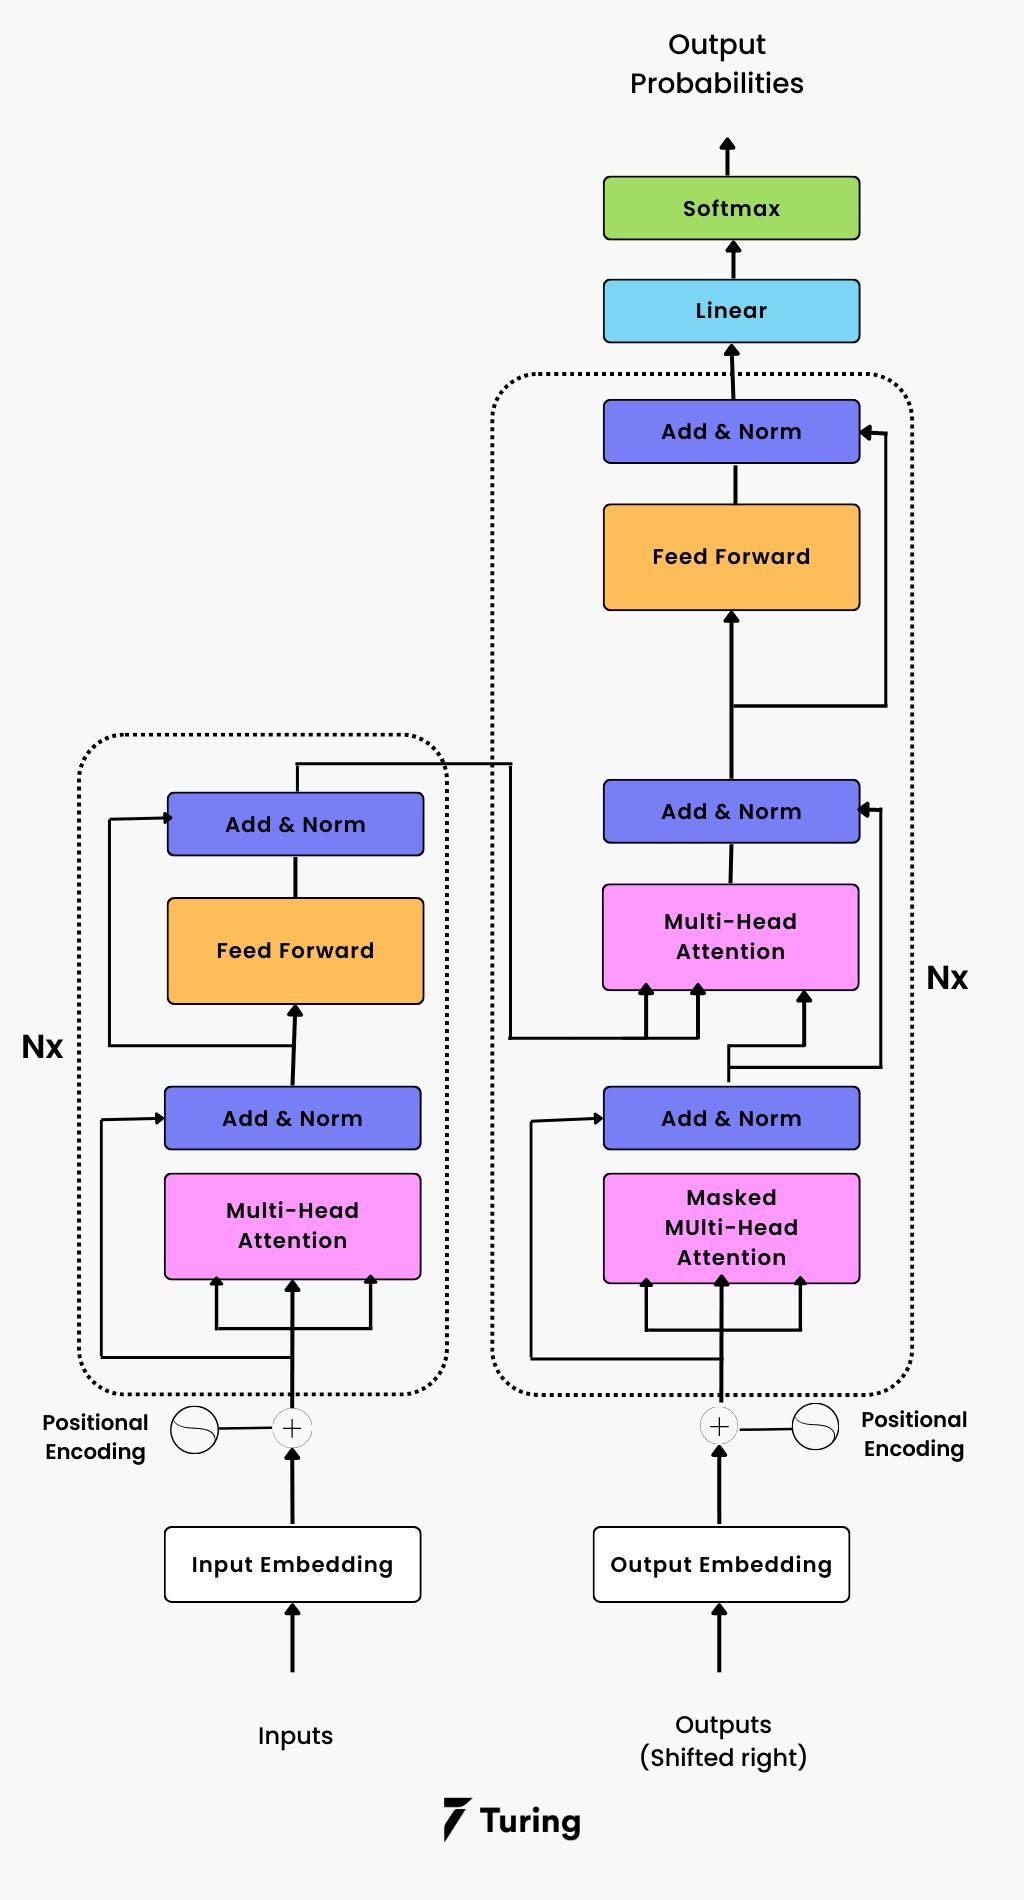
\includegraphics[width=8cm]{images/Transformer_architecture.png}
    \caption{Kiến trúc Transformer}
    \end{figure*}

\section{Mục tiêu}
Mục tiêu của notebook này là để chứng minh cách các Mô hình Ngôn ngữ Lớn (Large Language Models - LLMs) có thể được sử dụng cho một số tác vụ liên quan đến xử lý ngôn ngữ (language processing). Trong trường hợp này, tôi sẽ tận dụng sức mạnh của học chuyển giao (transfer learning) để xây dựng một mô hình có khả năng tóm tắt các cuộc hội thoại (summarizing dialogues).

Nếu các bạn có thể chưa biết, transfer learning là một kỹ thuật học máy (machine learning technique) trong đó chúng ta sử dụng một mô hình được đào tạo trước (pre-trained model) - vốn đã có kiến thức trong một lĩnh vực rộng - và điều chỉnh chuyên môn của nó cho một tác vụ cụ thể (specific task) bằng cách huấn luyện nó trong một tập dữ liệu cụ thể (specific dataset) mà chúng ta có thể có. Quá trình này cũng có thể được gọi là tinh chỉnh (fine-tuning).

Thư viện Transformers - một trong những thư viện phổ biến nhất để làm việc với các tác vụ học sâu (deep learning tasks) - cung cấp khả năng làm việc với các kiến trúc (architectures) sau:\\

\begin{figure*}[htp]
    \centering
    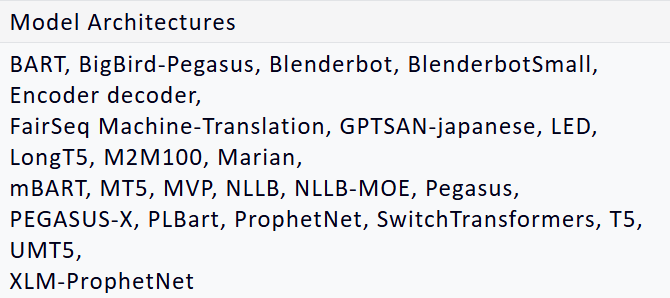
\includegraphics{images/kdl2.png}
    \caption{Các kiến trúc mô hình mà thư viện Transformers hỗ trợ}
    \end{figure*}

Thư viện Transformers cho phép chúng ta dễ dàng tải xuống và tinh chỉnh các mô hình được đào tạo trước tiên tiến, đồng thời cho phép chúng ta dễ dàng làm việc với cả TensorFlow và PyTorch cho một số tác vụ liên quan đến Xử lý Ngôn ngữ Tự nhiên (Natural Language Preprocessing - NLP), Thị giác Máy tính (Computer Vision), Âm thanh (Audio), v.v.
